\footnotesize
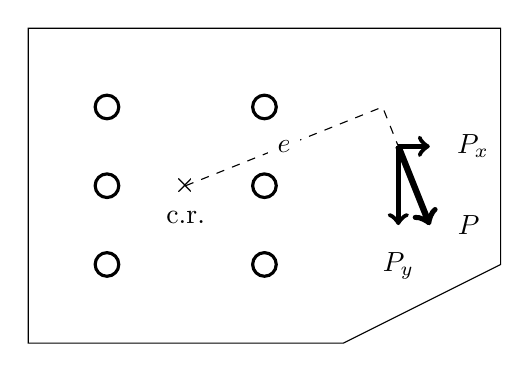
\begin{tikzpicture}
\draw(-1,-1)--++(4,0)--++(2,1)--++(0,3)-|cycle;
\foreach\x in{0,2}{
\foreach\y in{0,1,2}{
\node[circle,inner sep=0pt,minimum size=3mm,line width=.4mm,draw]at(\x,\y){};}}
\draw(1,1)node{\texttimes}node[below=2mm]{c.r.};
\draw[dashed](1,1)--++(2.5,1)node[fill=white,midway]{$e$}--++(.2,-.5)coordinate(A);
\draw[->,line width=.8mm](A)--++(.4,-1)node[right=2mm]{$P$};
\draw[->,line width=.6mm](A)--++(.4,0)node[right=2mm]{$P_x$};
\draw[->,line width=.6mm](A)--++(0,-1)node[below=2mm]{$P_y$};
\end{tikzpicture}